\documentclass{./../../Latex/handout}
\begin{document}
\thispagestyle{plain}
\myheader{Problem Set 4 Solutions}
\rhead{Problem Set 4 Solutions}

\textit{Type up your answers in a Word document and then save it as PDF before uploading them to Canvas. 
}

\begin{enumerate}
\item (2 pts) I regressed wealth on parents' wealth and found an $R^2=0.64$. What does this mean? Does a high $R^2$ imply that I am identifying the causal impact of parents' wealth on children's wealth? 
\item[] \textit{Answer}: An $R^2$ of 0.64 means that parents' wealth can explain 64\% of the variation in children's wealth in this model. However, a high $R^2$ does not establish the causal impact of parents' wealth on children's wealth. To make such a causal claim, we need to assume exogeneity, meaning that unobserved factors affecting an individual's wealth are uncorrelated with parents' wealth. However, this assumption may not hold in this case, as children with wealthier parents may have access to better educational opportunities, contributing to their ability to generate more wealth.   \\

\item (1 pt) Consider the following linear regression model:
$$ Y = \beta_0 + \beta_1 X + u $$
Show that $E(u|X)=0$ implies  $E(Y|X) = \beta_0 + \beta_1 X $. 
\item[] \textit{Answer}: By taking the conditional expectation of $Y = \beta_0 + \beta_1 X + u$ we can write:
$$ E(Y|X) = \beta_0 + \beta_1 X + E(u|X) $$
Once we substitute $E(u|X)=0$ into the previous equation, we obtain $E(Y|X) = \beta_0 + \beta_1 X$. \\~\\

% Question: Napping
\item (3 pts) A study was conducted to investigate the effects of short naps on memory. The study involved 200 participants who were allowed to nap for either 30 or 60 minutes. After waking up, each participant took a short test on short-term recall. The nap duration for each participant was randomly assigned based on a coin flip. Let $Y_i$ denote the score of the $i$'th participant on the test $(0 ≤ Y_i ≤ 100)$, and let $X_i$ denote the length of time the participant slept before the test ($X_i = $ 30 or 60). Consider the following regression model: $$ Y_i = \beta_0 + \beta_1 X_i + u_i $$ 
\begin{enumerate}
  \item Explain what the term $u_i$ represents. Why might different participants have different values of $u_i$?
  \item[] \textit{Answer}: $u_i$ represents the error term, which captures the effect of all other factors that influence the score $Y_i$ but are not included in the model. These factors could include an individual's cognitive ability or motivation, or distractions during the test. 
  
  Participants may have different values of $u_i$ because of individual differences in the unobserved factors that influence their short-term recall. For example, one participant may be more motivated to perform well on the test than another, leading to a higher score.  \\
  \item Do you think here $E(u_i|X_i) =0$? Why or why not? Will the estimated coefficients be biased or unbiased? 
  \item[] \textit{Answer}: Yes, the assumption $E(u_i|X_i) =0$ is satisfied here. Since the participants were randomly assigned to either a 30-minute or 60-minute nap, nap duration should be uncorrelated with unobserved factors affecting short-term recall. Under this assumption, the estimated coefficients will be unbiased.	\\
\item The estimated regression is $ \hat{Y}_i = 55 + 0.17 X_i $. Compute the predicted score for a participant who napped for 30 minutes and for a participant who napped for 60 minutes. Compute the estimated gain/loss in score from a longer nap. 
\item[] \textit{Answer}: $$ \hat{Y}_{X_i=30} = 55 + 0.17 \cdot 30 = 60.1  $$
	$$ \hat{Y}_{X_i=60} = 55 + 0.17 \cdot 60 = 65.2 $$
	So the estimated gain of the longer nap is: $65.2-60.1=5.1$. Note that we could have alternatively found this as $0.17\times 30$ because $0.17$ is the estimated impact on the score for an additional minute.\\
\end{enumerate}

% Question: R-output
\item (3 pts) 
Output from three regression models is presented below. 
\begin{center}
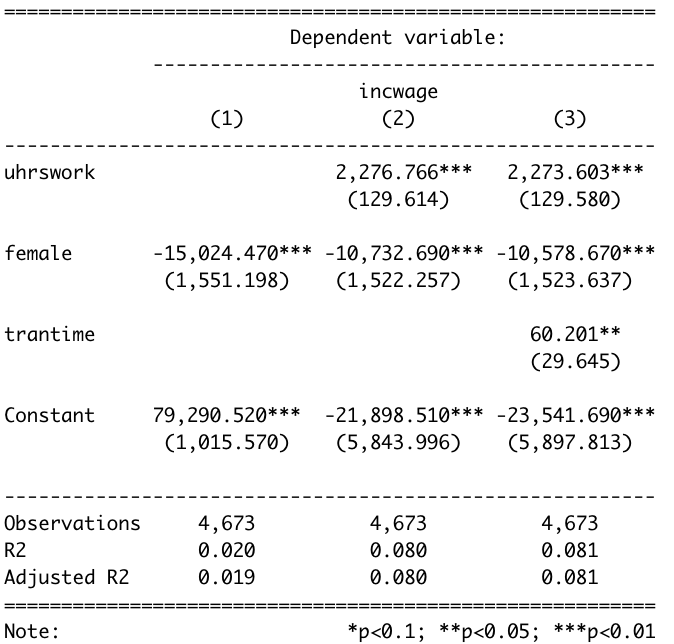
\includegraphics[scale=0.55]{reg.png} 	
\end{center}

The three models are as follows: 
\begin{align*}
	 \text{Model 1:} \quad incwage &=\beta_0 + \beta_1  female + u \\
	 \text{Model 2:} \quad incwage &=\beta_0 + \beta_1  female + \beta_2 uhrswork + u \\
	 \text{Model 3:} \quad incwage &=\beta_0 + \beta_1  female + \beta_2 uhrswork + \beta_3 trantime + u 
\end{align*}

The variables are defined as follows:
\begin{itemize}
  \item \textit{incwage}: annual wage and salary income (in \$)
  \item \textit{female}: indicator variable that takes value 1 for females and 0 for males
  \item \textit{uhrswork}: hours worked each week
  \item \textit{trantime}: transit time to work (in minutes) \\
\end{itemize}

Answer the following questions (0.5 pts each):
\begin{enumerate}
  \item Interpret the coefficient on \textit{female} in Model 1. Is this coefficient statistically significant at a 1\% level of significance?
  \item[] \textit{Answer}: On average, in our sample, annual wages for women are \\ \$15,024.47 lower than for men. This coefficient is statistically significant at 1\% level of significance as the $p$-value is less than 0.01 (as indicated by the triple-asterisks.) Since the coefficient is significant at 1\% level of significance, it is also significant at any $\alpha>0.01$ level of significance. \\
  
  \item Interpret the coefficient on \textit{female} from Model 2.
  \item[] \textit{Answer}: Keeping the weekly number of hours worked constant, the average annual wages for women in our sample are \$10,732.69 lower than those of men.	\\
  
  \item In the second model, we added the variable for hours worked, and the coefficient on \textit{female} went down considerably. Given this pattern, do you think women work more or fewer hours than men in our sample? (Note: The coefficient on \textit{uhrswork} is positive.)
  \item[] \textit{Answer}: By adding hours worked as an explanatory variable to our model, we find that the gender wage gap decreases. This implies that a portion of the gap estimated in Model 1 can be attributed to differences in the number of hours worked by men and women. However, when we control for hours worked and compare wages between men and women, we observe a smaller gap in pay. This suggests that, on average, men tend to work more hours each week than women, which contributes to their higher annual wages. \\
  
  \item Interpret the coefficient on \textit{trantime} in model three. If I wanted to test the null hypothesis that $\beta_3=0$, what would be the associated $t$-value for this test?
  \item[] \textit{Answer}: On average, each additional minute of transit time to work is associated with an increase of \$60.2 in annual income, keeping all else constant. If we wanted to test the hypothesis that $\beta_3=0$. Our $t$-value for this test would be:
  $$ t_0 = \frac{\hat{\beta}_3}{SE_{\hat{\beta_3}}} = \frac{60.201}{29.645} = 2.03 $$	\\
  
  \item Find the $p$-value for the $t$-statistic you found in (d).\footnote{You need to refer to the standard normal table or use \texttt{2 * (1 - pnorm(abs(t)))} in R.} What does this $p$-value tell us?
  \item[] \textit{Answer}: The associated $p$-value is given by:
  $$ p = 2 P(Z < -t_0) =  2 \times 0.0212 = 0.0424$$
  This means that the coefficient on \textit{trantime} is significant at 4.24\% level of significance. (Note that since $p=0.0424$, \textit{trantime} is significant at 5\% but not 1\% level of significance, hence two asterisks instead of three.)	\\
  
  \item Does the inclusion of \textit{trantime} improve the explanatory power of the regression model for predicting wages? Why or why not?
  \item[] \textit{Answer}: The increase in adjusted $R^2$ from 0.08 to 0.081 with the inclusion of \textit{trantime} in the regression model is very small. This suggests that the additional explanatory power provided by including transit time is negligible.	\\
\end{enumerate}
Pay attention to the units of measurement of each variable while interpreting the coefficients. \\

\item (1 pt) Consider the following regression model:
$$ wages_i =\beta_0 +  \beta_1  experience_i + \beta_2 immigrant_i +  \beta_3  experience_i \times immigrant_i + u $$
where $immigrant_i$ is a binary variable that takes the value 1 if an individual is an immigrant and 0 otherwise. $wages_i$ captures earnings and $experience_i$ captures work experience. \\
What is the interpretation of $\beta_3$?  (Hint: Take the expectation of the equation conditional on $immigrant_i=1$ and $immigrant_i=0$.)
\item[] \textit{Answer}: Note that we will assume: $$E(u_i | immigrant_i=1)=E(u | immigrant_i=0)=0$$
Under the previous assumption, 
\begin{align*}
	E(wages_i| immigrant_i=1) &= (\beta_0 + \beta_2)  +  (\beta_1+\beta_3)  experience_i \\
	E(wages_i| immigrant_i=0) &=\beta_0 +  \beta_1  experience_i 
\end{align*}
From here, we can see that $\beta_3$ tells us by how much the impact of experience on wages differs between immigrants and non-immigrants. 
\end{enumerate}
\end{document}